\documentclass[11pt, a4paper]{article}
\usepackage{pdfpages}
\usepackage{parallel}
\usepackage[T2A]{fontenc}
\usepackage{ucs}
\usepackage[utf8x]{inputenc}
\usepackage[polish,english,russian]{babel}
\usepackage{hyperref}
\usepackage{rotating}
\usepackage[inner=2cm,top=1.8cm,outer=2cm,bottom=2.3cm,nohead]{geometry}
\usepackage{listings}
\usepackage{graphicx}
\usepackage{wrapfig}
\usepackage{longtable}
\usepackage{indentfirst}
\usepackage{array}
\usepackage{tikzsymbols}
\usepackage{soul}
\usepackage[ruled,vlined]{algorithm2e}
%\counterwithout{figure}{section} 

\usepackage{url}
\makeatletter
\g@addto@macro{\UrlBreaks}{\UrlOrds}
\makeatother

\newcolumntype{P}[1]{>{\raggedright\arraybackslash}p{#1}}
\frenchspacing
\usepackage{fixltx2e} %text sub- and superscripts
\usepackage{icomma} % коскі ў матэматычным рэжыме
\PreloadUnicodePage{4}

\newcommand{\longpage}{\enlargethispage{\baselineskip}}
\newcommand{\shortpage}{\enlargethispage{-\baselineskip}}

\def\switchlang#1{\expandafter\csname switchlang#1\endcsname}
\def\switchlangbe{
\let\saverefname=\refname%
\def\refname{Літаратура}%
\def\figurename{Іл.}%
}
\def\switchlangen{
\let\saverefname=\refname%
\def\refname{References}%
\def\figurename{Fig.}%
}
\def\switchlangru{
\let\saverefname=\refname%
\let\savefigurename=\figurename%
\def\refname{Литература}%
\def\figurename{Рис.}%
}

\hyphenation{admi-ni-stra-tive}
\hyphenation{ex-pe-ri-ence}
\hyphenation{fle-xi-bi-li-ty}
\hyphenation{Py-thon}
\hyphenation{ma-the-ma-ti-cal}
\hyphenation{re-ported}
\hyphenation{imp-le-menta-tions}
\hyphenation{pro-vides}
\hyphenation{en-gi-neering}
\hyphenation{com-pa-ti-bi-li-ty}
\hyphenation{im-pos-sible}
\hyphenation{desk-top}
\hyphenation{elec-tro-nic}
\hyphenation{com-pa-ny}
\hyphenation{de-ve-lop-ment}
\hyphenation{de-ve-loping}
\hyphenation{de-ve-lop}
\hyphenation{da-ta-ba-se}
\hyphenation{plat-forms}
\hyphenation{or-ga-ni-za-tion}
\hyphenation{pro-gramming}
\hyphenation{in-stru-ments}
\hyphenation{Li-nux}
\hyphenation{sour-ce}
\hyphenation{en-vi-ron-ment}
\hyphenation{Te-le-pathy}
\hyphenation{Li-nux-ov-ka}
\hyphenation{Open-BSD}
\hyphenation{Free-BSD}
\hyphenation{men-ti-on-ed}
\hyphenation{app-li-ca-tion}

\def\progref!#1!{\texttt{#1}}
\renewcommand{\arraystretch}{2} %Іначай формулы ў матрыцы зліпаюцца з лініямі
\usepackage{array}

\def\interview #1 (#2), #3, #4, #5\par{

\section[#1, #3, #4]{#1 -- #3, #4}
\def\qname{LVEE}
\def\aname{#1}
\def\q ##1\par{{\noindent \bf \qname: ##1 }\par}
\def\a{{\noindent \bf \aname: } \def\qname{L}\def\aname{#2}}
}

\def\interview* #1 (#2), #3, #4, #5\par{

\section*{#1\\{\small\rm #3, #4. #5}}
\ifx\ParallelWhichBox\undefined%
    \addcontentsline{toc}{section}{#1, #3, #4}%
\else%
\ifnum\ParallelWhichBox=0%
    \addcontentsline{toc}{section}{#1, #3, #4}%
\fi\fi%

\def\qname{LVEE}
\def\aname{#1}
\def\q ##1\par{{\noindent \bf \qname: ##1 }\par}
\def\a{{\noindent \bf \aname: } \def\qname{L}\def\aname{#2}}
}

\newcommand{\interviewfooter}[1]{
\vskip 1em
\noindent \textit{#1}
}

\switchlang{ru}
\begin{document}

\title{1996 "--- Kensington Expert Mouse Trackball 5.0}
\date{}
\maketitle
\selectlanguage{russian}
В 1996 году Kensington выпустила пятую по счёту модель Expert Mouse Trackball. Трекбол претерпел существенный редизайн \cite{KensingtonPC}. В то время как предыдущие модели были достаточно классическими двухкнопочными устройствами, Expert Mouse Trackball 5.0 оказался оснащен шаром большего диаметра и четырьмя крупными кнопками, симметрично расположенными вокруг шара по аналогии с лепестками цветка (рис. \ref{fig:ExpertMousePic}).

\begin{figure}[h]
    \centering
    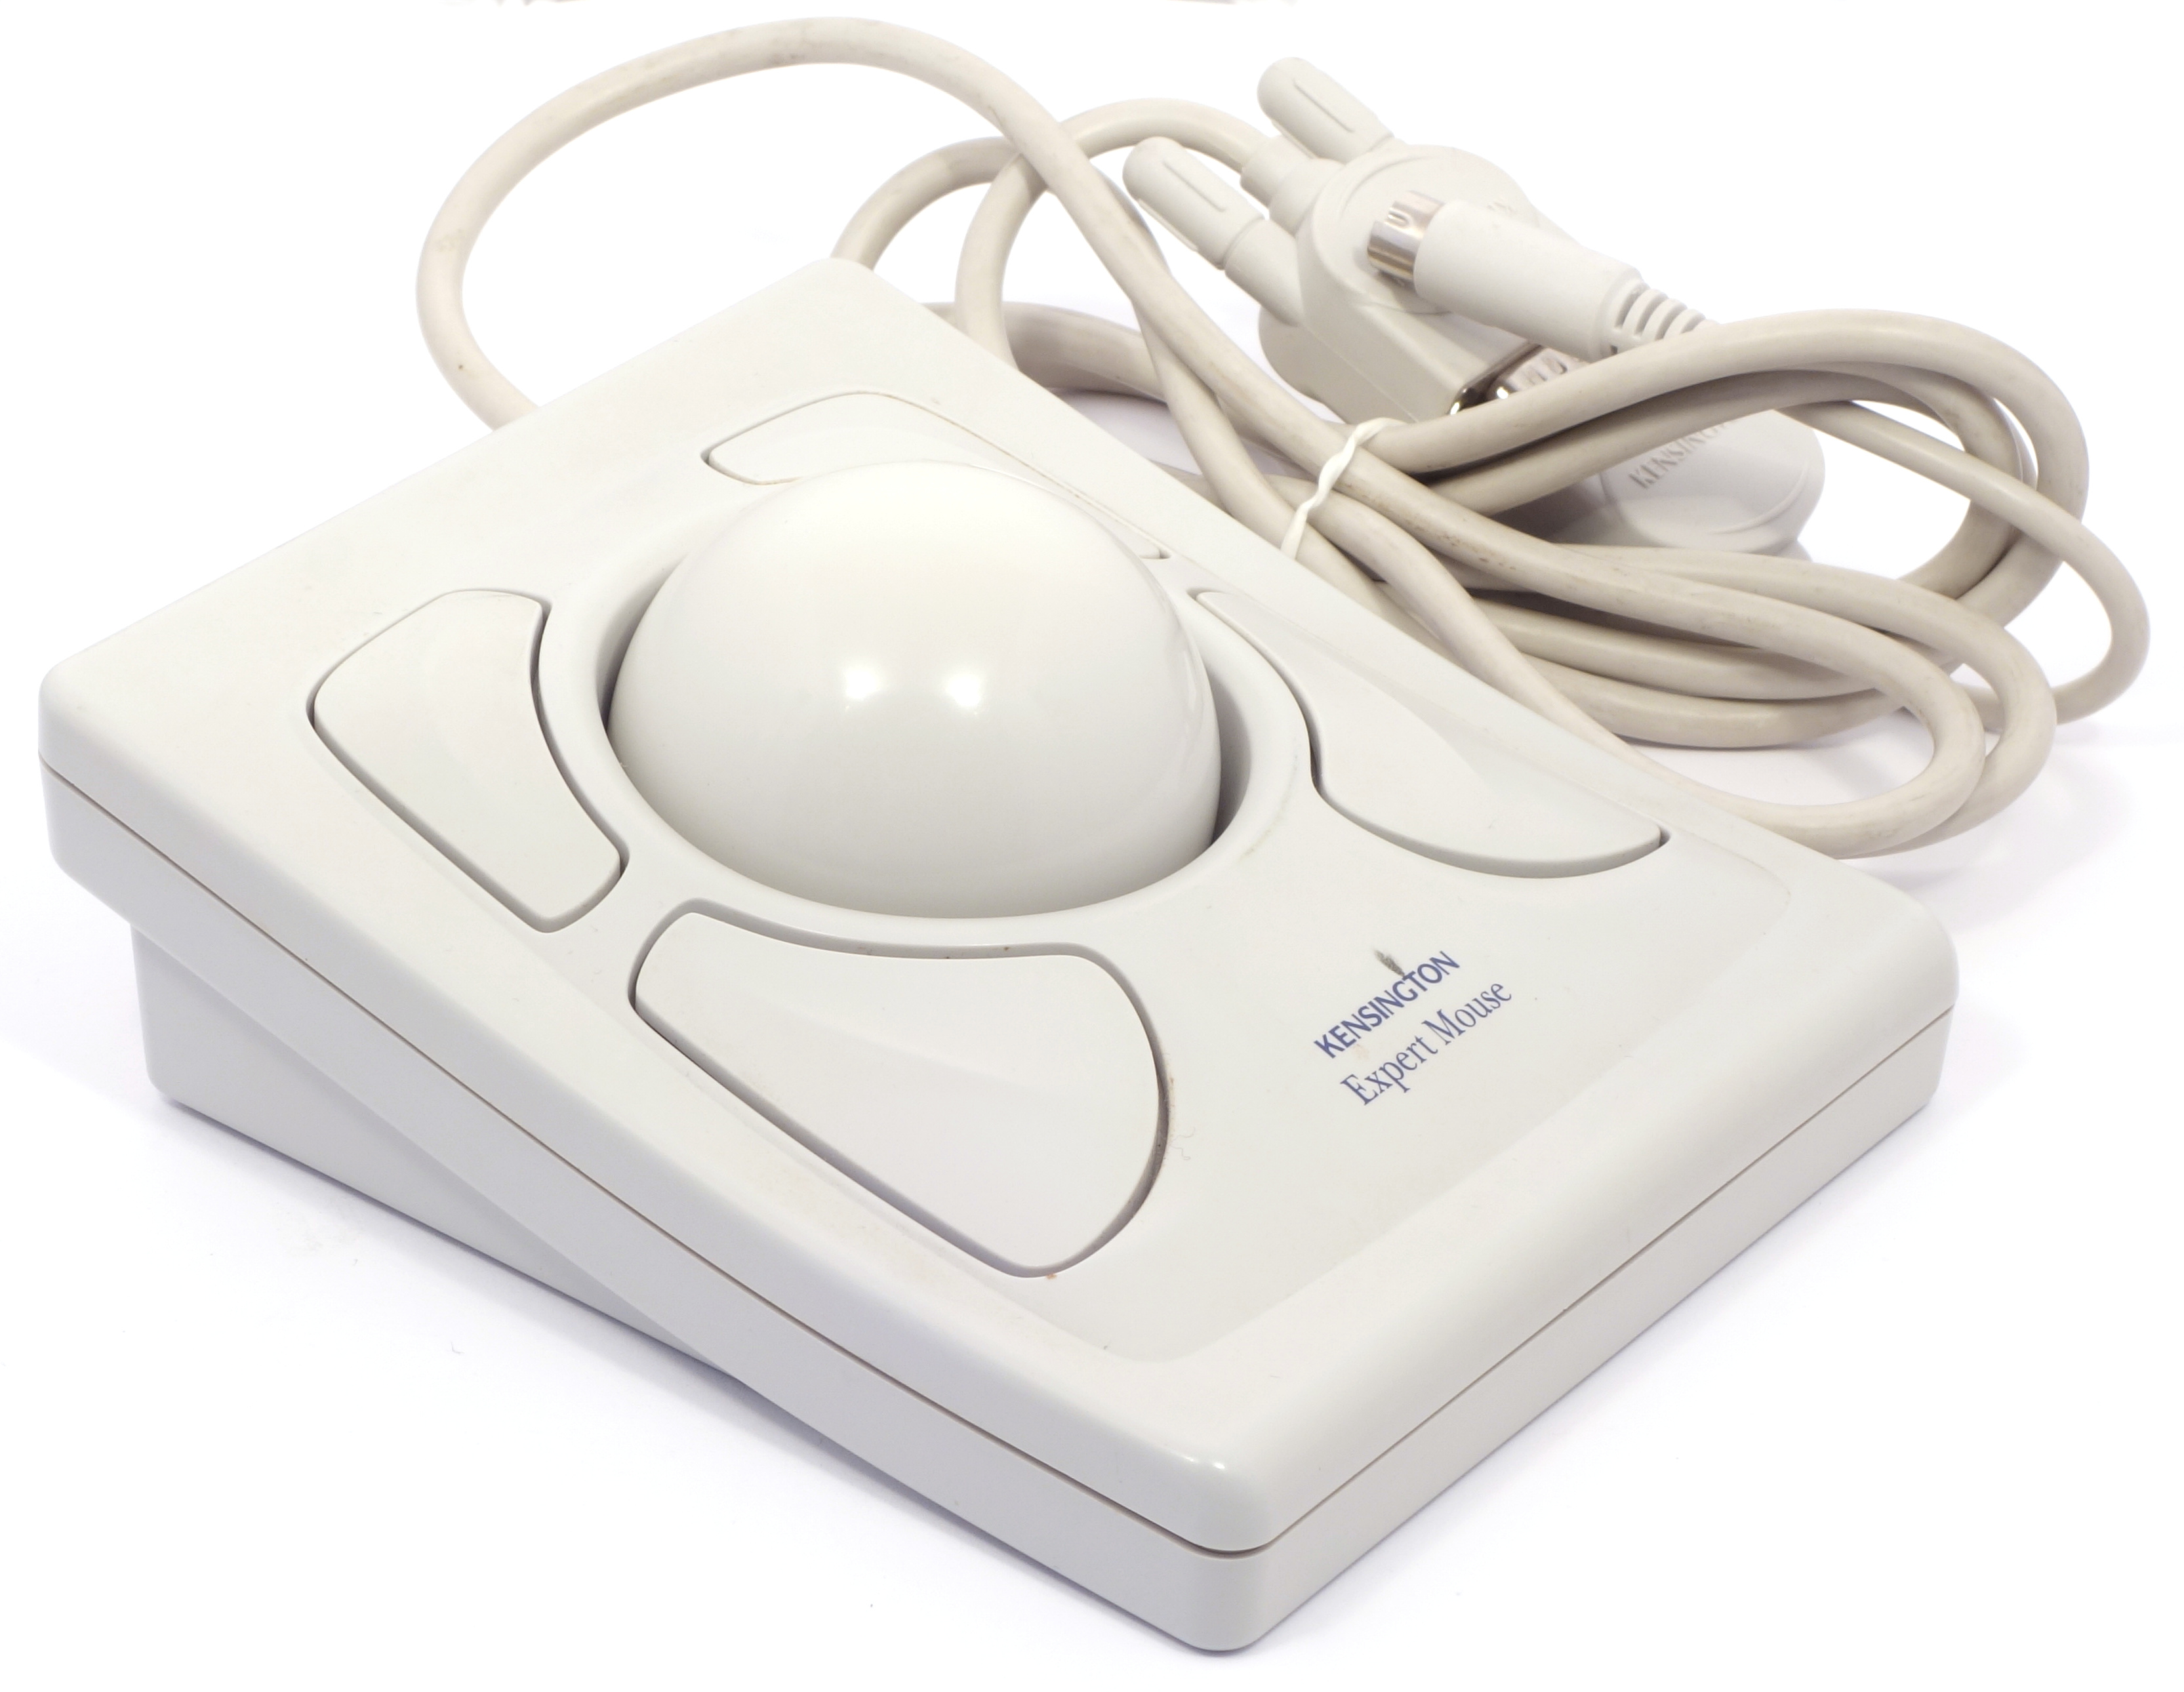
\includegraphics[scale=0.4]{1996_kensington_expert_trackball_5/pic_60.jpg}
    \caption{Kensington Expert Trackball}
    \label{fig:ExpertMousePic}
\end{figure}

Для Macintosh была выпущена аналогичная модель с предсказуемым названием Turbo Mouse 5.0 \cite{KensingtonMac} и интерфейсом ADB, в то время как Expert Mouse комплектовался сменными кабелями для подключения к последовательному интерфейсу и к порту PS/2 (также отдельно выпускалась шинная версия с ISA-адаптером). Визуально Turbo Mouse была идентична, воспроизводя тот же самый <<цветочный>> стиль (рис. \ref{fig:ExpertMouseTopBottom}).

\begin{figure}[h]
    \centering
    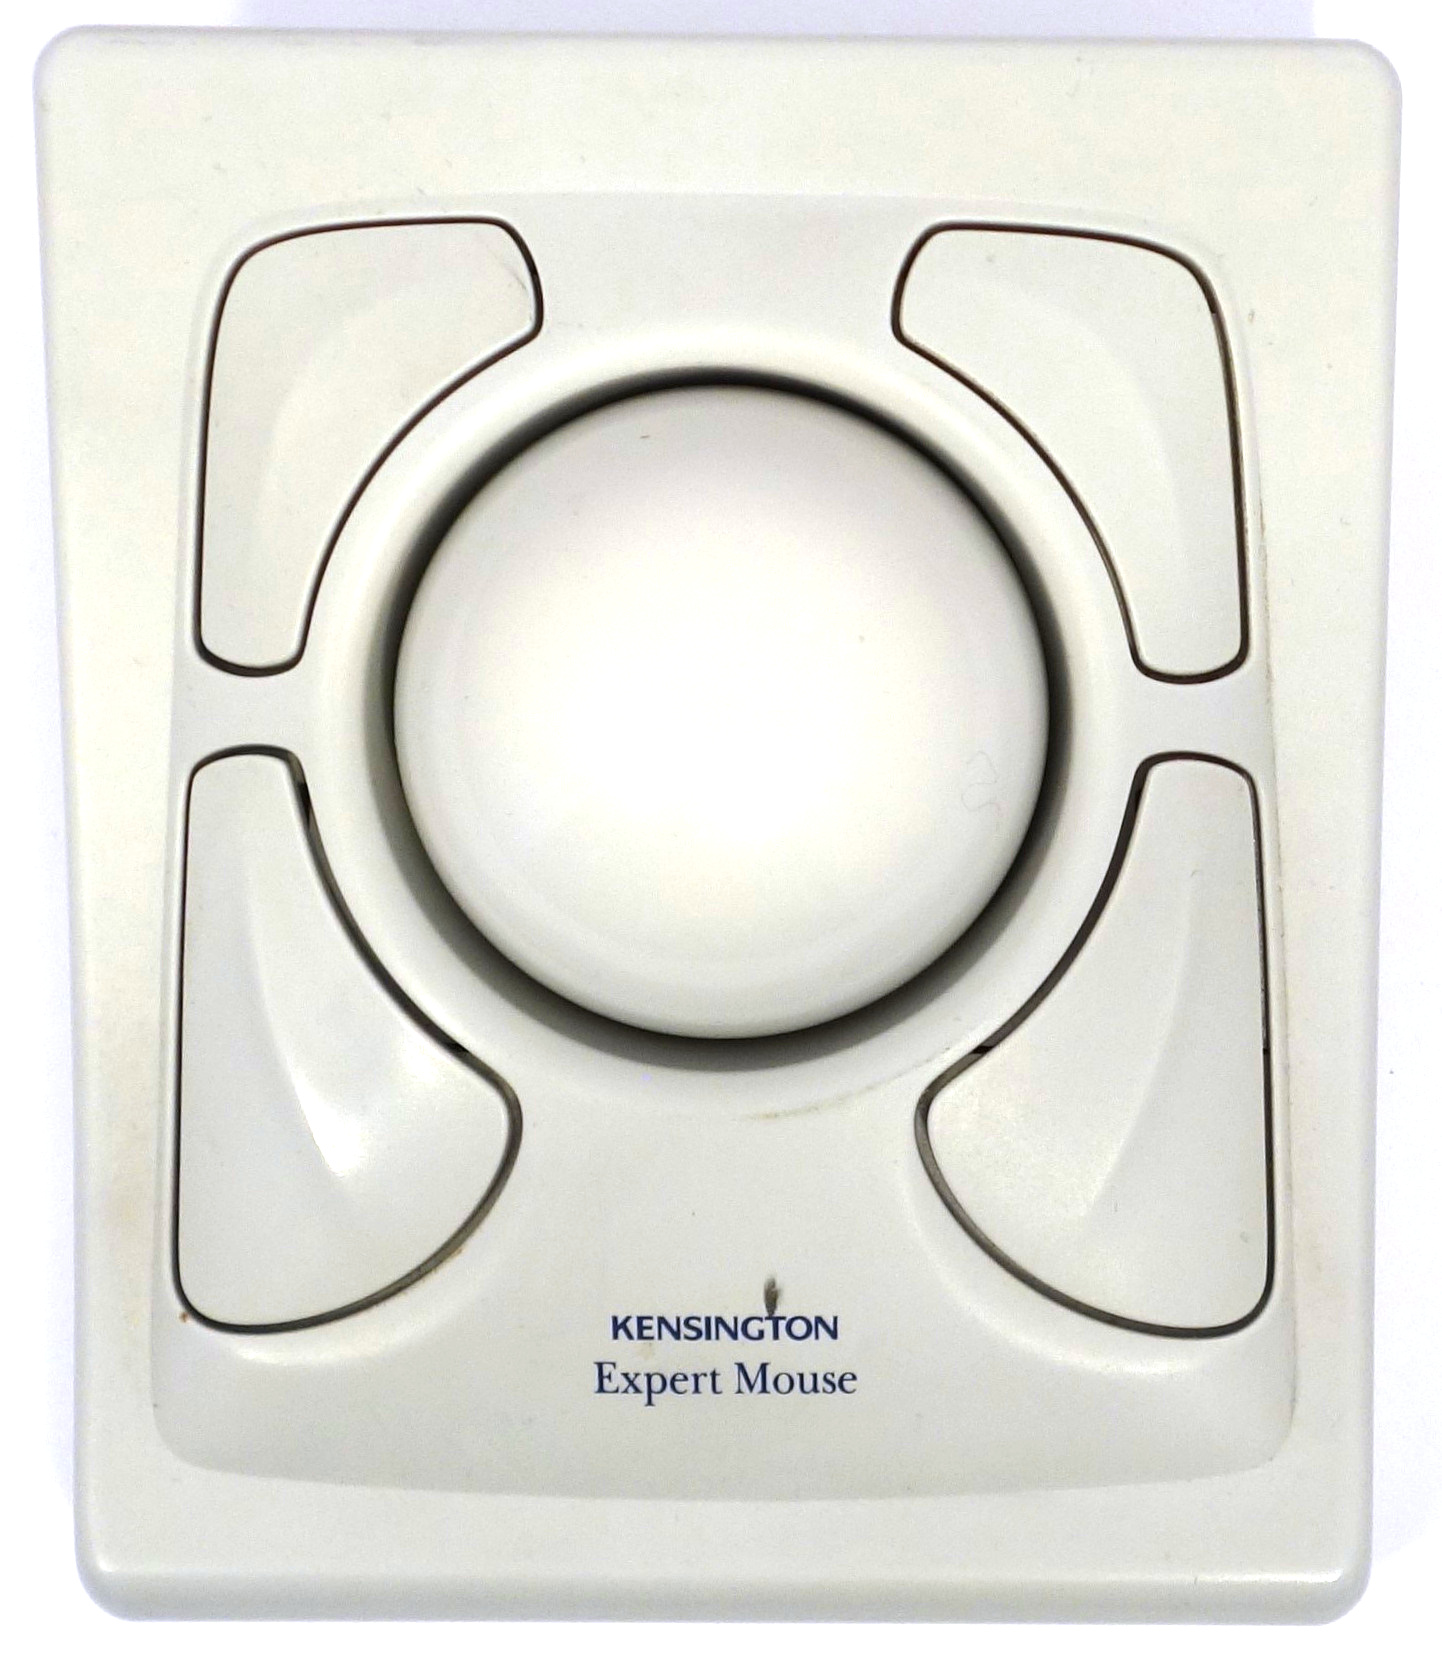
\includegraphics[scale=0.4]{1996_kensington_expert_trackball_5/top_30.jpg}
    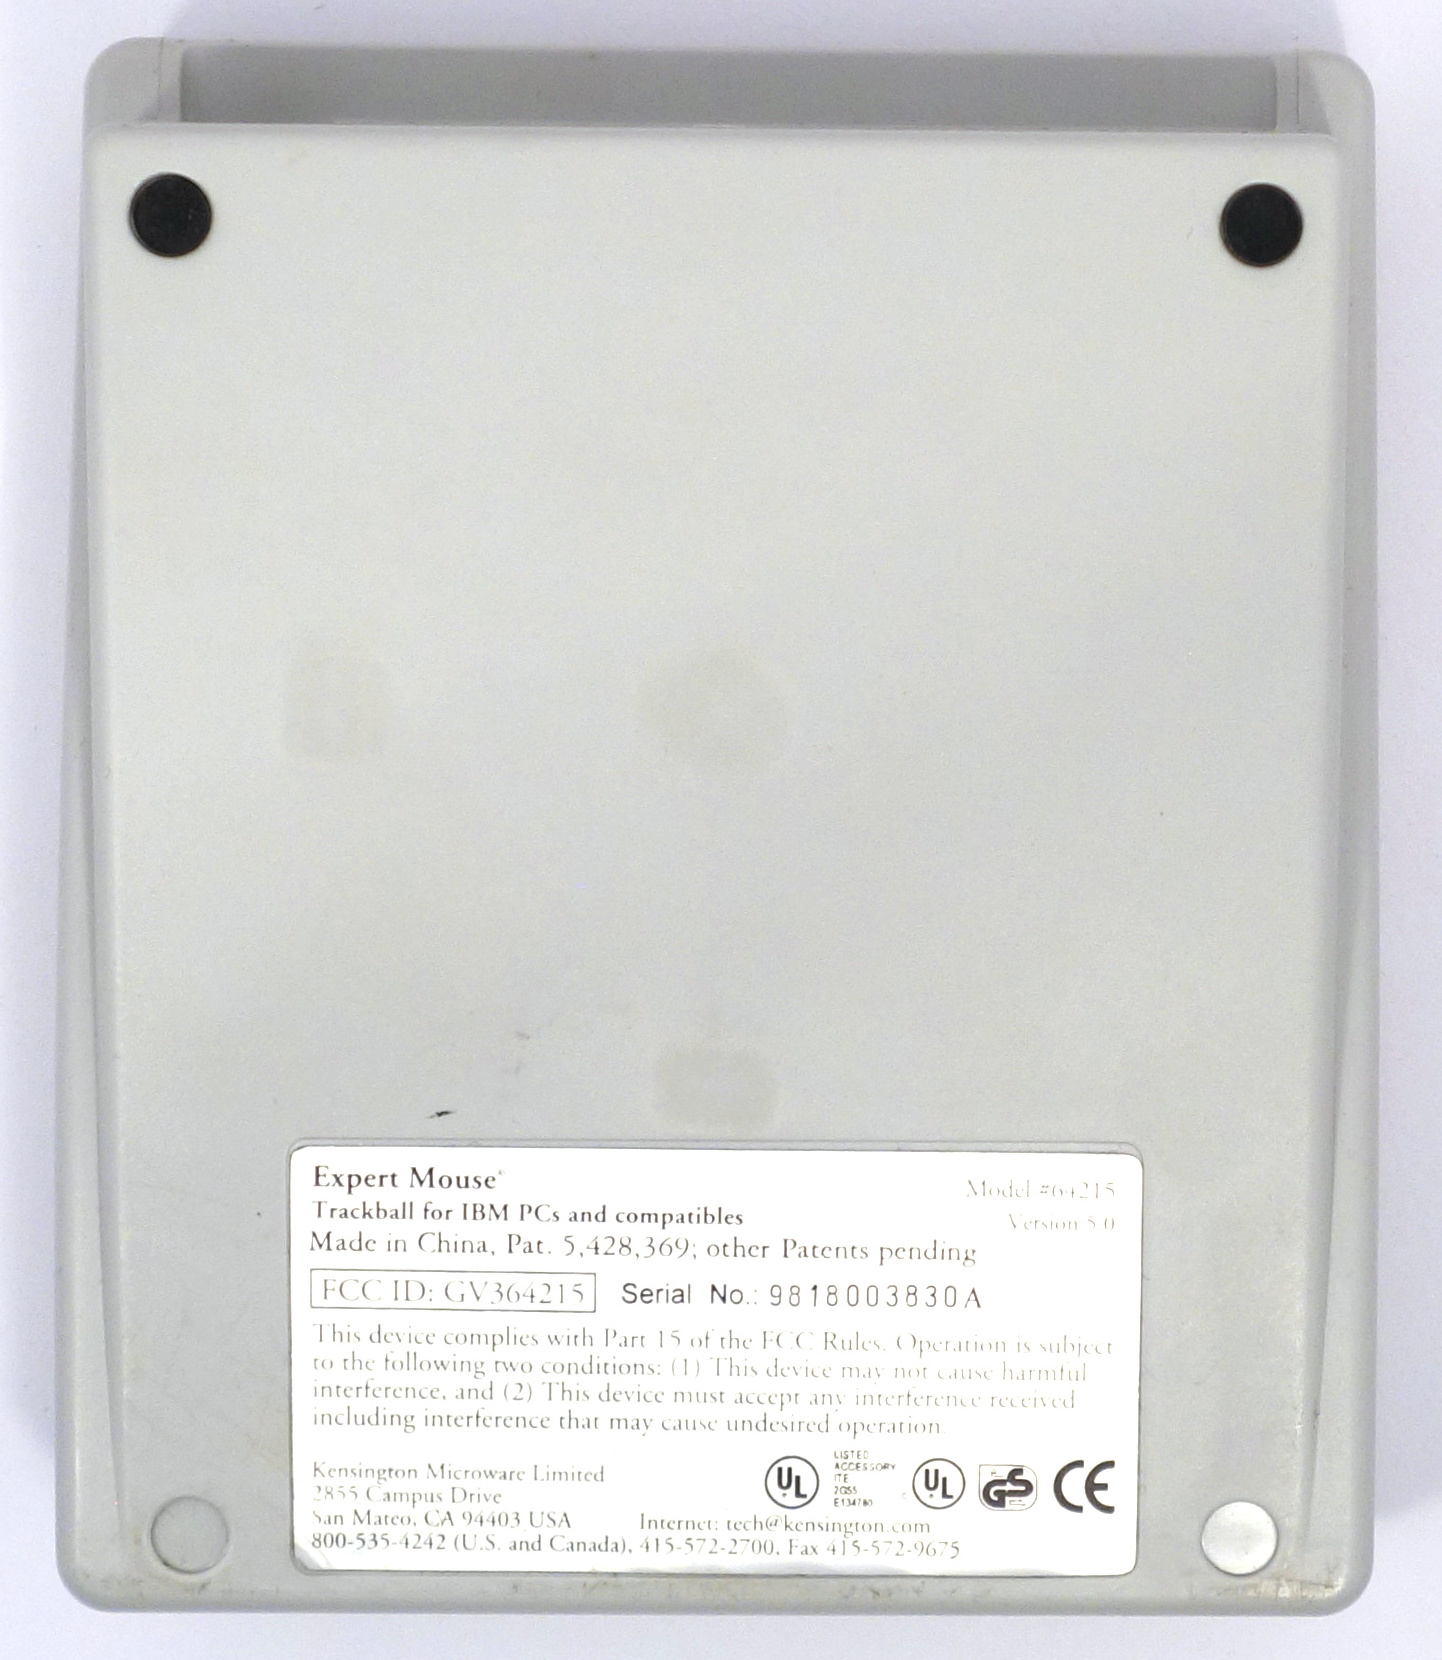
\includegraphics[scale=0.4]{1996_kensington_expert_trackball_5/bottom_30.jpg}
    \caption{Kensington Expert Mouse Trackball вид сверху}
    \label{fig:ExpertMouseTopBottom}
\end{figure}

Несмотря на большой шар и крупные кнопки, Expert Mouse Trackball является не самым габаритным устройством (рис. \ref{fig:ExpertMouseSize}): фактически, полость для шара и кнопки занимают большую часть корпуса. Необычным является также то, что шар никак не закреплён и свободно лежит в сферической полости (поэтому, помимо флористических ассоциаций внешний вид трекбола также наводит на мысли о яйце в птичьем гнезде). Это значительно облегчает чистку устройства (но осложняет его переноску с места на место, поскольку  отклонение от горизонтального положения корпуса чревато падением шара).

\begin{figure}[h]
    \centering
    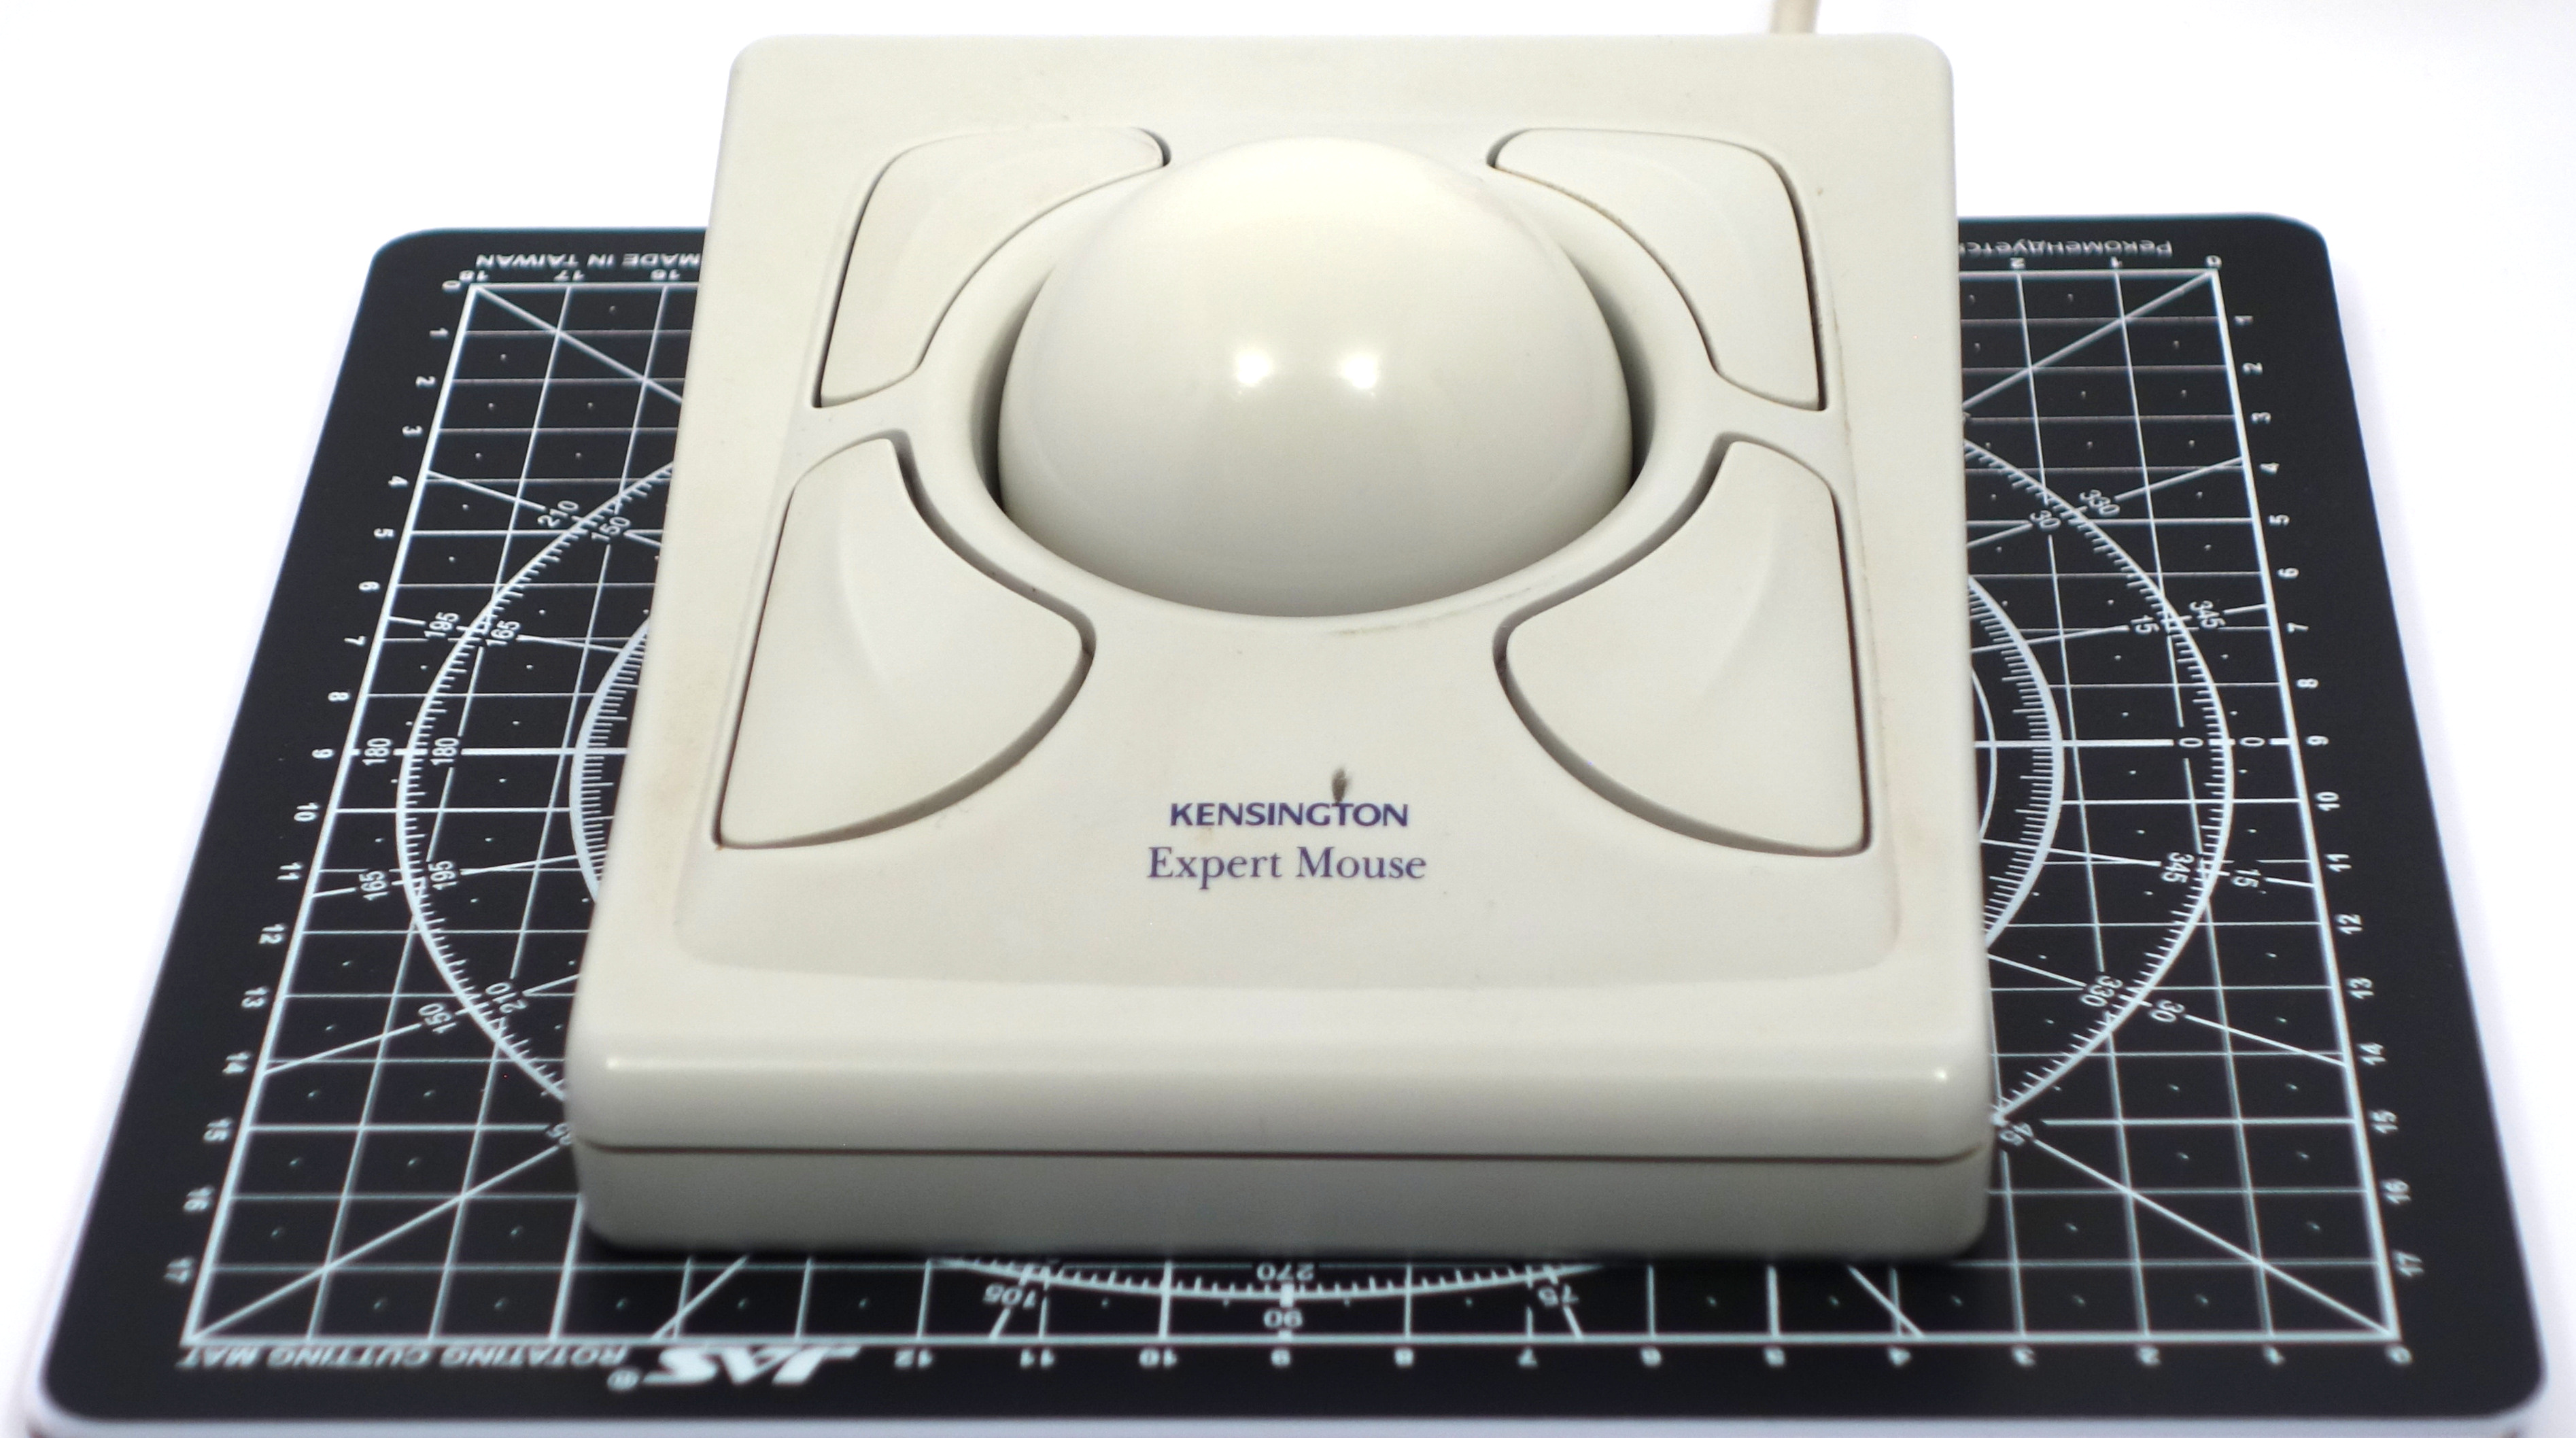
\includegraphics[scale=0.3]{1996_kensington_expert_trackball_5/size_30.jpg}
    \caption{Kensington Expert Mouse Trackball на размерном коврике с шагом сетки 1~см}
    \label{fig:ExpertMouseSize}
\end{figure}

Безусловно, шар такого диаметра рассчитан на прецизионное перемещение курсора, востребованное в САПР и графических редакторах (учитывая нестандартную дизайнерскую концепцию, можно предположить, что расчет делался в значительной степени на эту последнюю категорию). В плане эргономики необычное расположение кнопок оказывается достаточно удобным: при работе пользователь накрывает шар пальцами и, в зависимости от положения кисти, в состоянии дотянуться не перемещая руку либо до двух ближних, либо до одной ближней и двух дальних кнопок (рис. \ref{fig:ExpertMouseHand}). По умолчанию две ближние к пользователю (и имеющие наибольшую площадь) кнопки играют роль левой и правой кнопок мыши, что безусловно упрощает работу тем, кому дополнительные кнопки не требуются либо требуются редко. Положительной характеристикой эргономики устройства является и характерная для Kensington  симметричность корпуса, делающая его одинаково удобным как для левшей, так и для правшей.

\begin{figure}[h]
    \centering
    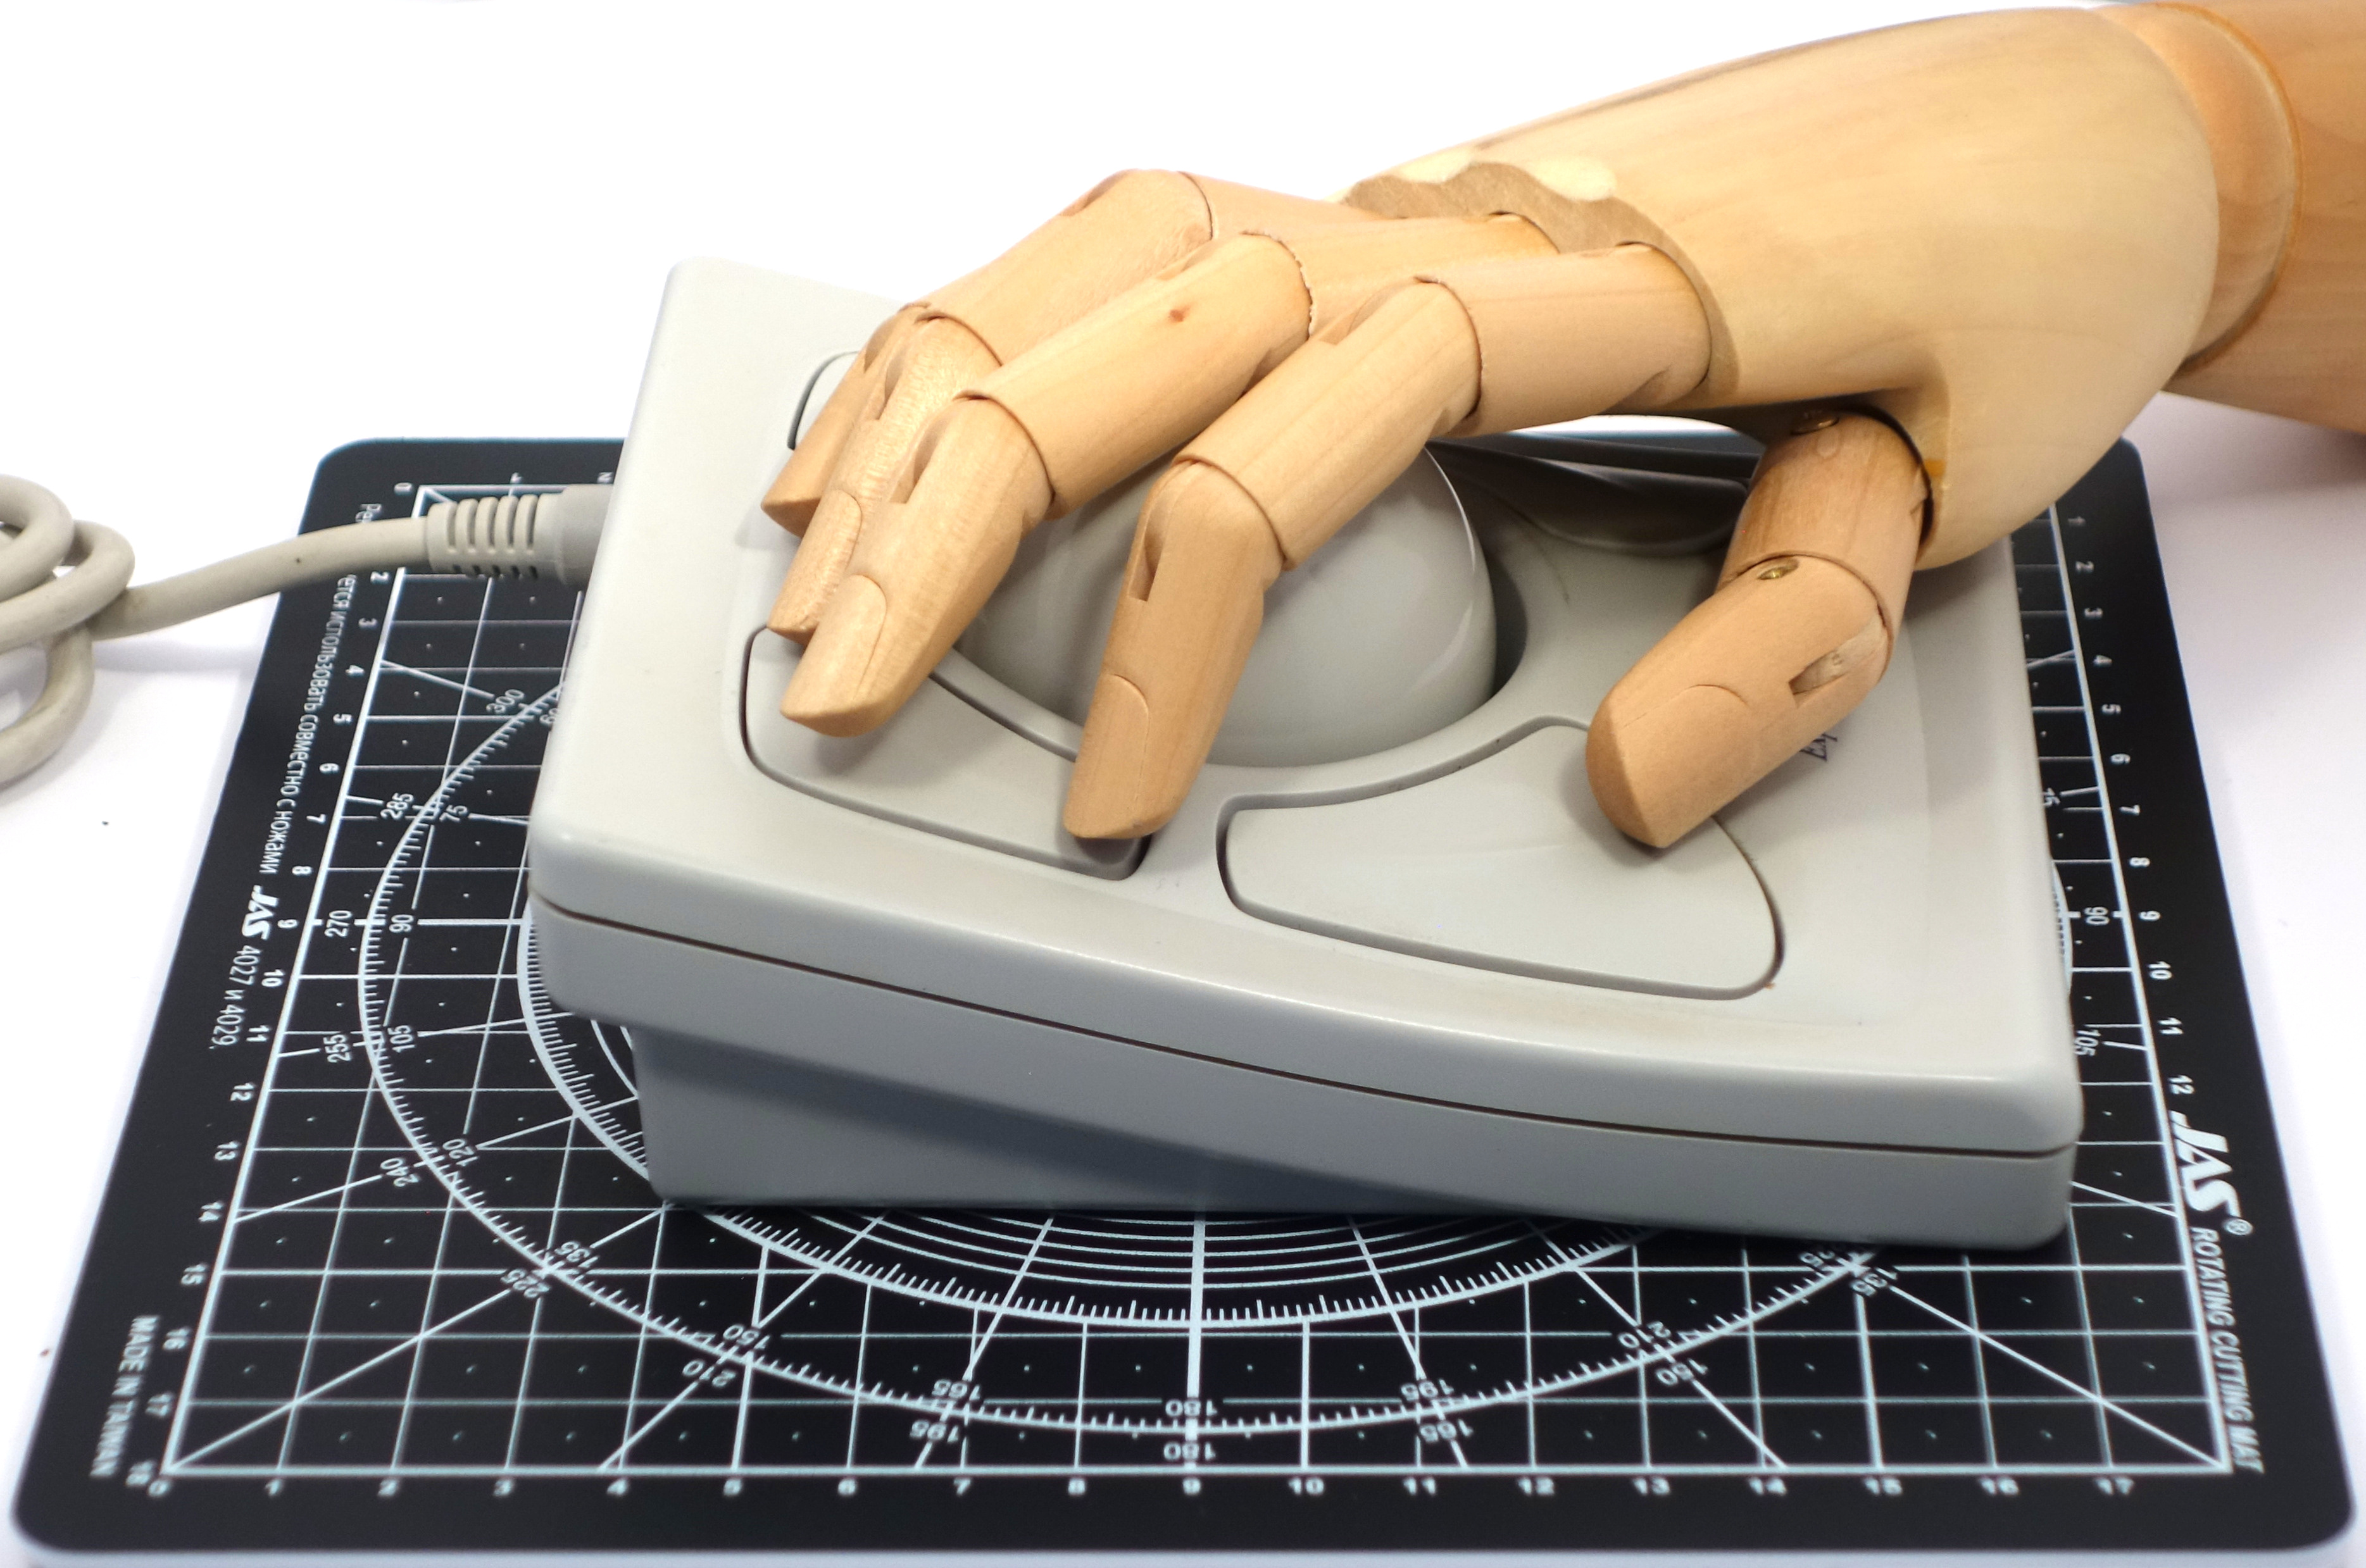
\includegraphics[scale=0.3]{1996_kensington_expert_trackball_5/hand_30.jpg}
    \caption{Изображение Kensington Expert Mouse Trackball с моделью руки человека}
    \label{fig:ExpertMouseHand}
\end{figure}

Изучение внутреннего устройства (рис. \ref{fig:ExpertMouseInside}) показывает, что устройство использует  оптомеханическое преобразование и высоконадежные металлические ролики. При этом оптомеханическое преобразование выполнено нестандартно, по запатентованной технологии <<оптического рычага>> (англ. optical levering) \cite{eu}: вместо используемой в большинстве устройств регистрирации света, прошедшего через прорези вращающегося диска, здесь регистрируется отражение от радиальных металлических <<ребер>>, расположенных на торце ролика "--- фактически, на боковой стороне подшипника, приводимого в движение вращением шара. Очевидно, плотная набивка ребер позволила разработчикам отказаться от диска, уменьшая тем самым габариты устройства без ущерба для его разрешающей способности. 

\begin{figure}[h]
    \centering
    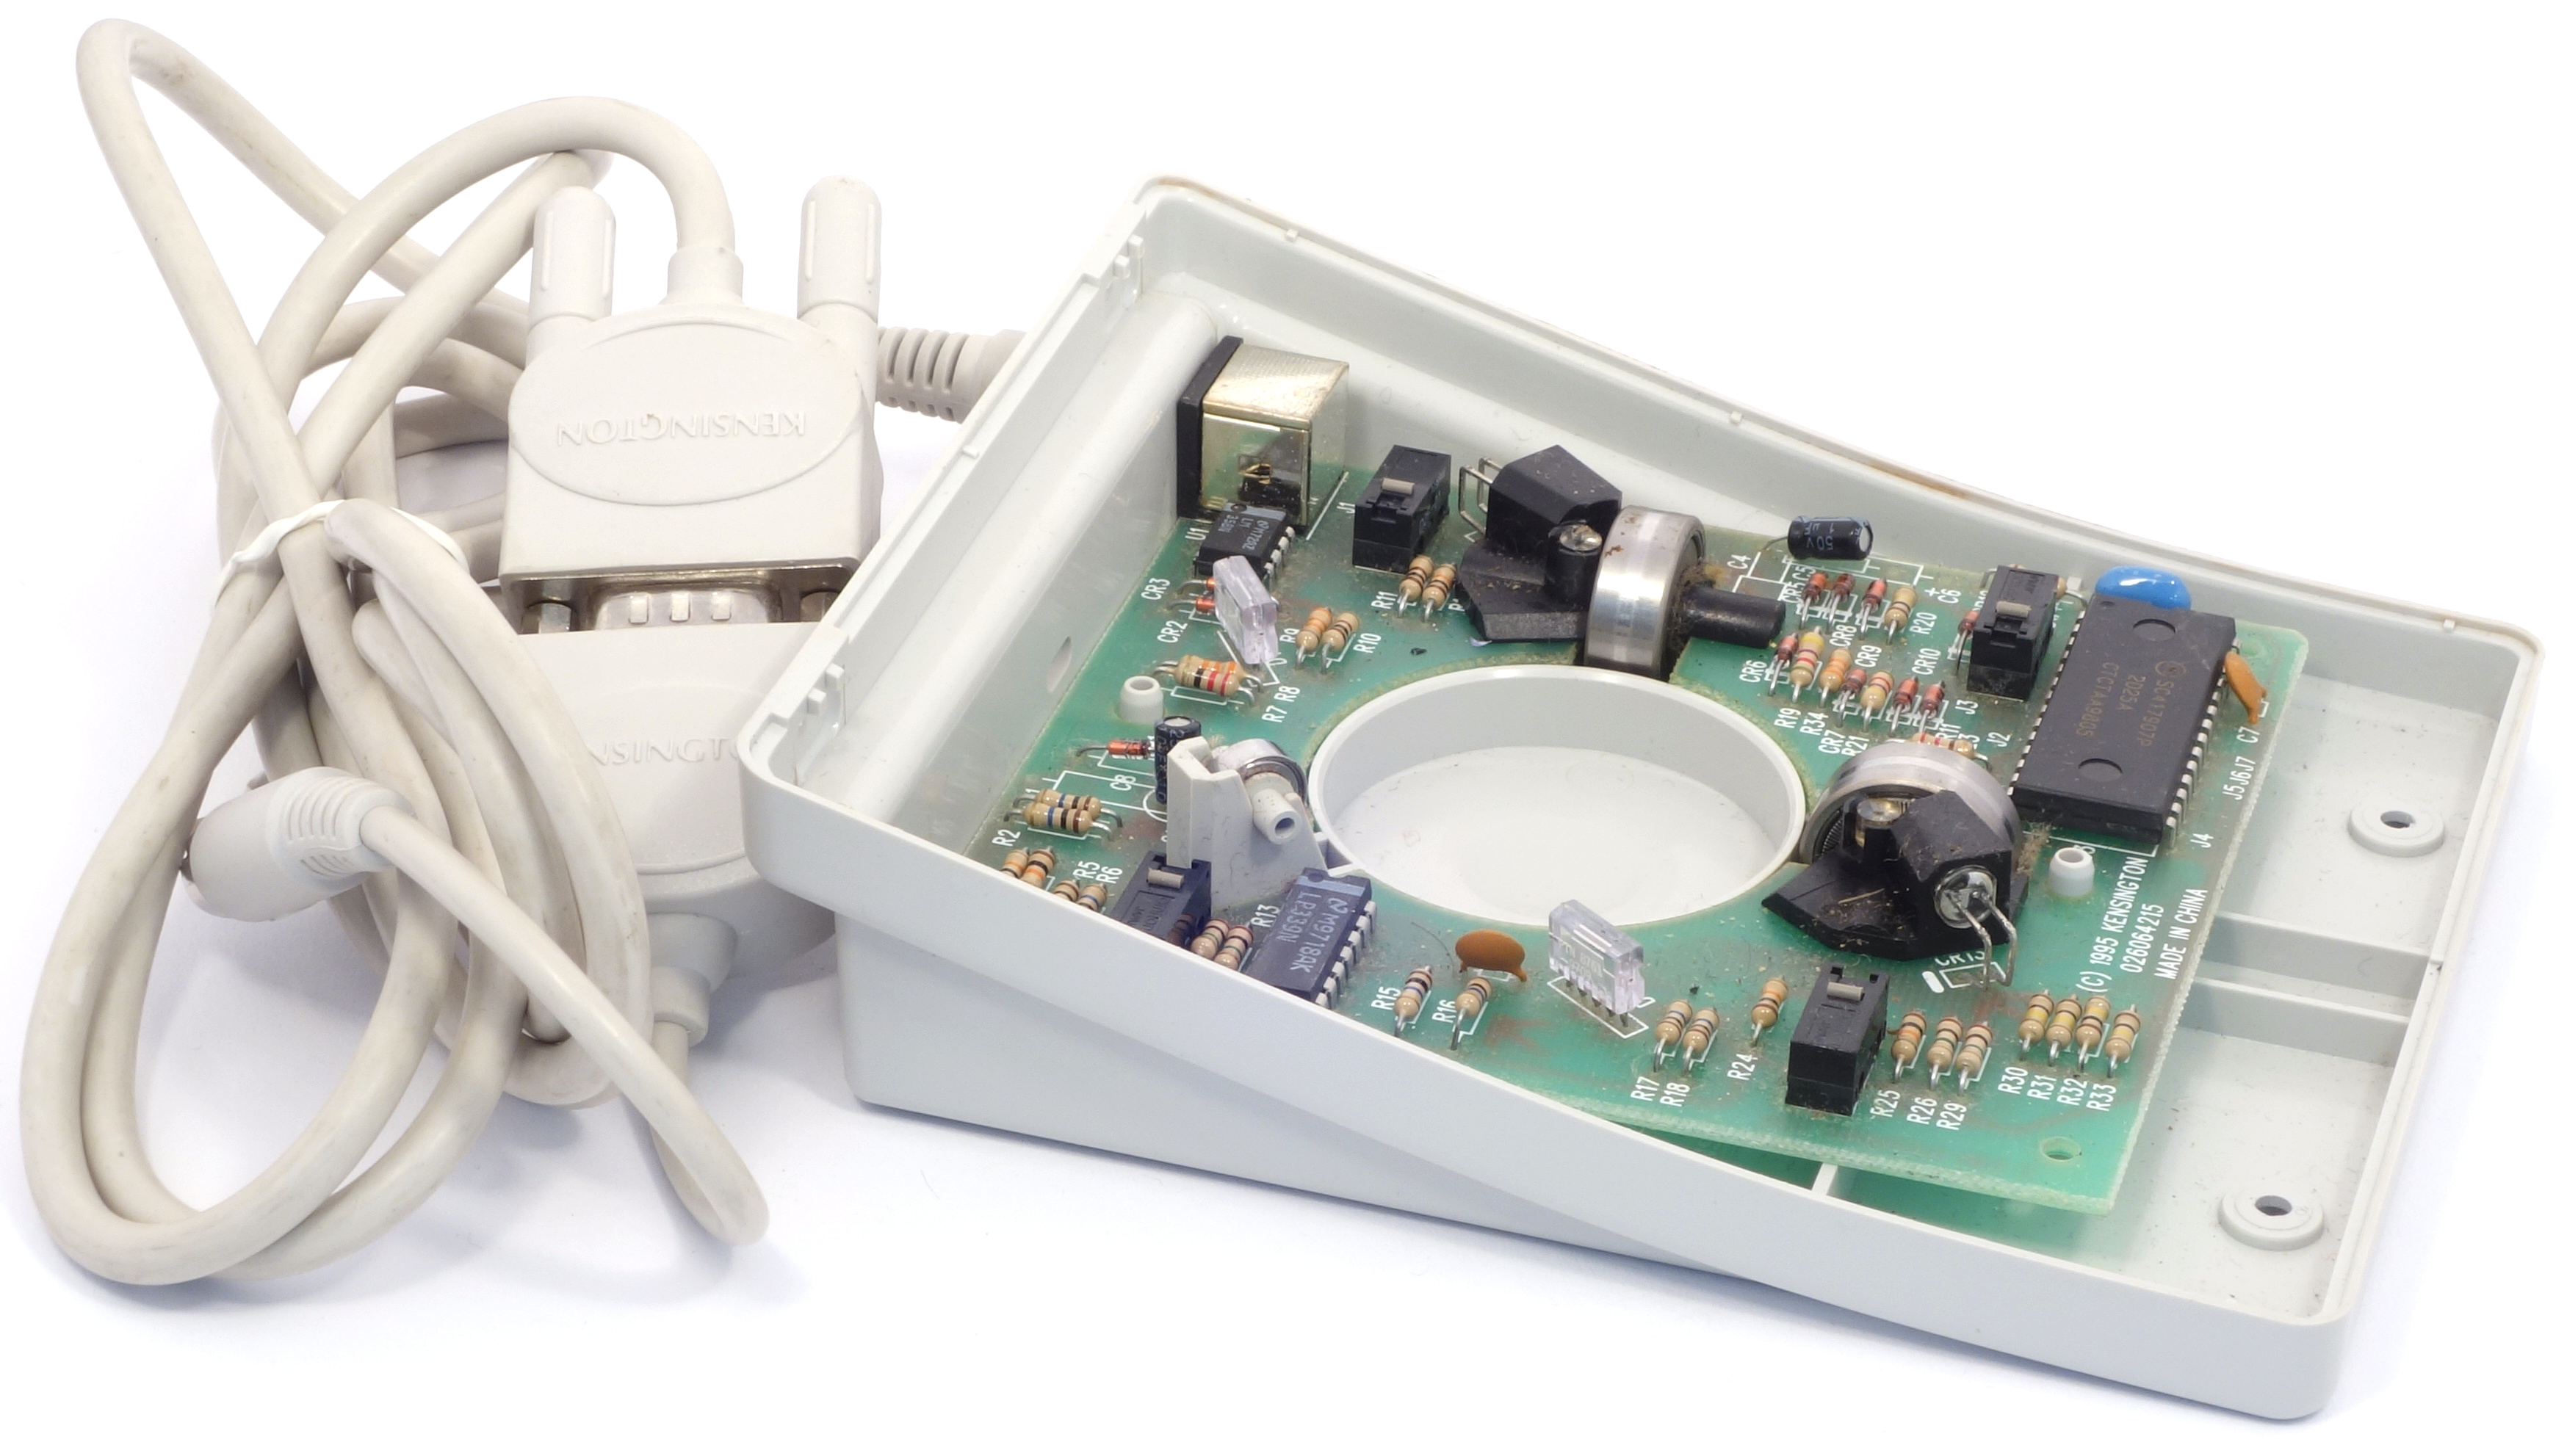
\includegraphics[scale=0.65]{1996_kensington_expert_trackball_5/inside_60.jpg}
    \caption{Kensington Expert Mouse Trackball в разобранном виде}
    \label{fig:ExpertMouseInside}
\end{figure}

\begin{thebibliography}{9}

\bibitem {KensingtonPC} Kensington: Expert Mouse 5.0 "--- \url{https://web.archive.org/web/19970106170305/http://www.kensington.com/prod/mice/mice3b.html}
\bibitem {KensingtonMac} Kensington: Turbo Mouse 5.0 "--- \url{https://web.archive.org/web/19970106170317/http://www.kensington.com/prod/mice/mice3a.html}
\bibitem {eu} Kensington -- Trackballs.EU "--- \url{https://web.archive.org/web/20210423041707/https://forum.trackballs.eu/viewtopic.php?f=14&t=43}
\end{thebibliography}

\end{document}
